% Created 2018-04-30 Mon 14:26
% Intended LaTeX compiler: pdflatex
\documentclass[t, aspectratio=169]{beamer}
\usepackage[utf8]{inputenc}
\usepackage[T1]{fontenc}
\usepackage{graphicx}
\usepackage{grffile}
\usepackage{longtable}
\usepackage{wrapfig}
\usepackage{rotating}
\usepackage[normalem]{ulem}
\usepackage{amsmath}
\usepackage{textcomp}
\usepackage{amssymb}
\usepackage{capt-of}
\usepackage{hyperref}
\usepackage{minted}
\usepackage{natbib}
\beamertemplatenavigationsymbolsempty
\BeforeBeginEnvironment{frame}{\subsection{}}
\usepackage[font=small,skip=0pt]{caption}
\usetheme[compress]{Amsterdam}
\author{Nathan Hughes}
\date{\today}
\title{Statistical Consulting For Biology}
\hypersetup{
 pdfauthor={Nathan Hughes},
 pdftitle={Statistical Consulting For Biology},
 pdfkeywords={},
 pdfsubject={},
 pdfcreator={Emacs 27.0.50 (Org mode 9.1.9)},
 pdflang={English}}
\begin{document}

\maketitle
\begin{frame}{Outline}
\tableofcontents
\end{frame}

\addtobeamertemplate{block begin}{%
  \setlength{\textwidth}{1.0\textwidth}%
}{}

\addtobeamertemplate{block alerted begin}{%
  \setlength{\textwidth}{1.0\textwidth}%
}{}

\addtobeamertemplate{block example begin}{%
  \setlength{\textwidth}{1.0\textwidth}%
}{}


\setbeamertemplate{caption}[numbered]
\setbeamerfont{bibliography item}{size=\footnotesize}
\setbeamerfont{bibliography entry author}{size=\footnotesize}
\setbeamerfont{bibliography entry title}{size=\footnotesize}
\setbeamerfont{bibliography entry location}{size=\footnotesize}
\setbeamerfont{bibliography entry note}{size=\footnotesize}
\setbeamertemplate{bibliography item}{\insertbiblabel}

\section{Intro}
\label{sec:orgeb8ac31}
\begin{frame}[label={sec:orged1f2d9}]{What was the data set}
\begin{block}{We focused on looking at a μCT image dataset}
\begin{itemize}
\item Its output (morphometric) data.
\item This was part of a Wheat (\emph{Triticum aestivum}) drought experiment.
\end{itemize}

\begin{center}
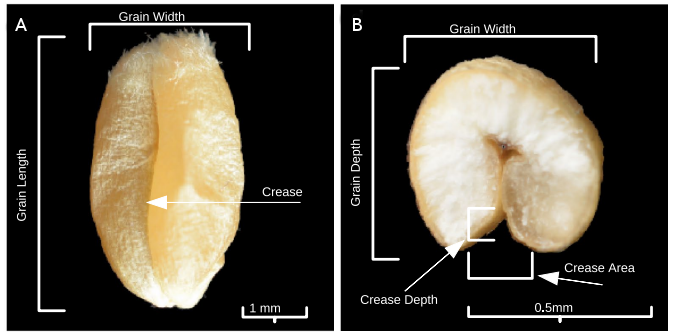
\includegraphics[width=7cm]{./seeds.png}
\end{center}
\end{block}
\end{frame}

\begin{frame}[label={sec:orgef2e2c6}]{Experiment Details}
\begin{block}{Drought Experiment Parameters}
\begin{longtable}{l|l}
\alert{Normal Watering} & \alert{Droughted}\\
\hline
\endfirsthead
\multicolumn{2}{l}{Continued from previous page} \\
\hline

\alert{Normal Watering} & \alert{Droughted} \\

\hline
\endhead
\hline\multicolumn{2}{r}{Continued on next page} \\
\endfoot
\endlastfoot
\hline
25C & 25C\\
30C & 30C\\
35C & 35C\\
\end{longtable}
\end{block}
\end{frame}


\section{Working as a group}
\label{sec:orgcbe63bb}
\begin{frame}[label={sec:org4bd19e5}]{Working as a group}
\begin{block}{Insight}
\begin{itemize}
\item I was already very familiar with the data
\item Which  meant I was too close to it to be "open-minded"
\end{itemize}
\end{block}
\end{frame}

\begin{frame}[label={sec:org0fec998}]{Benefits of discussing the data}
\begin{block}{Explaining teaches}
\begin{itemize}
\item Going through and explaining data makes you re-evaluate it
\item Stops you taking data for granted!
\item Helps you recognise your own mistakes and misunderstandings
\end{itemize}
\end{block}
\end{frame}

\begin{frame}[label={sec:orgc9d53ed}]{Benefits of discussing the data}
\begin{block}{Analysis is a living and evolving process}
\begin{itemize}
\item "Individuals and interactions over processes and tools"
\begin{itemize}
\item Kent Beck \emph{et al}.
\end{itemize}
\end{itemize}
\end{block}
\end{frame}

\begin{frame}[label={sec:org976f079}]{Group discussion}
\begin{block}{Suggestions}
\begin{itemize}
\item Our group suggested that Principal Component Analysis would be well suited to the data
\begin{itemize}
\item It may provide a method of looking at which traits are most effected by the experiment treatments
\end{itemize}
\item Another idea was using MANOVA to explore mean differences in treatments
\end{itemize}
\end{block}
\end{frame}


\section{Presenting Data}
\label{sec:org0d2ebad}
\begin{frame}[label={sec:org30b408d}]{Presenting the data}
\begin{block}{Interest in how best you could convey information}
\begin{itemize}
\item We looked at the data from a visualisation point of view
\item How you could show details on morphometric phenotypes in concise charts, plots or diagrams
\item We knew that some of the data couldn't be used, but not \emph{why}
\end{itemize}
\end{block}
\end{frame}
\begin{frame}[label={sec:org6db41f6}]{Showing the errors in the data}
\begin{center}
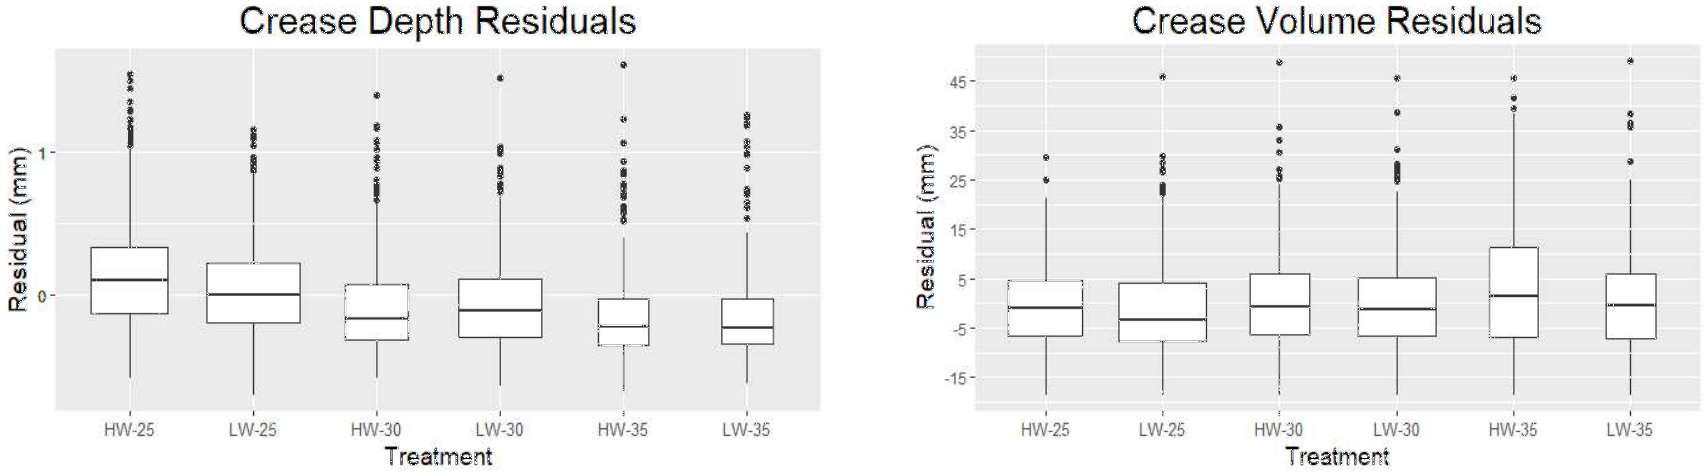
\includegraphics[width=14cm]{./peter.png}
\end{center}
\end{frame}

\begin{frame}[label={sec:org4bfa1f7}]{Showing relationships of traits}
\begin{center}
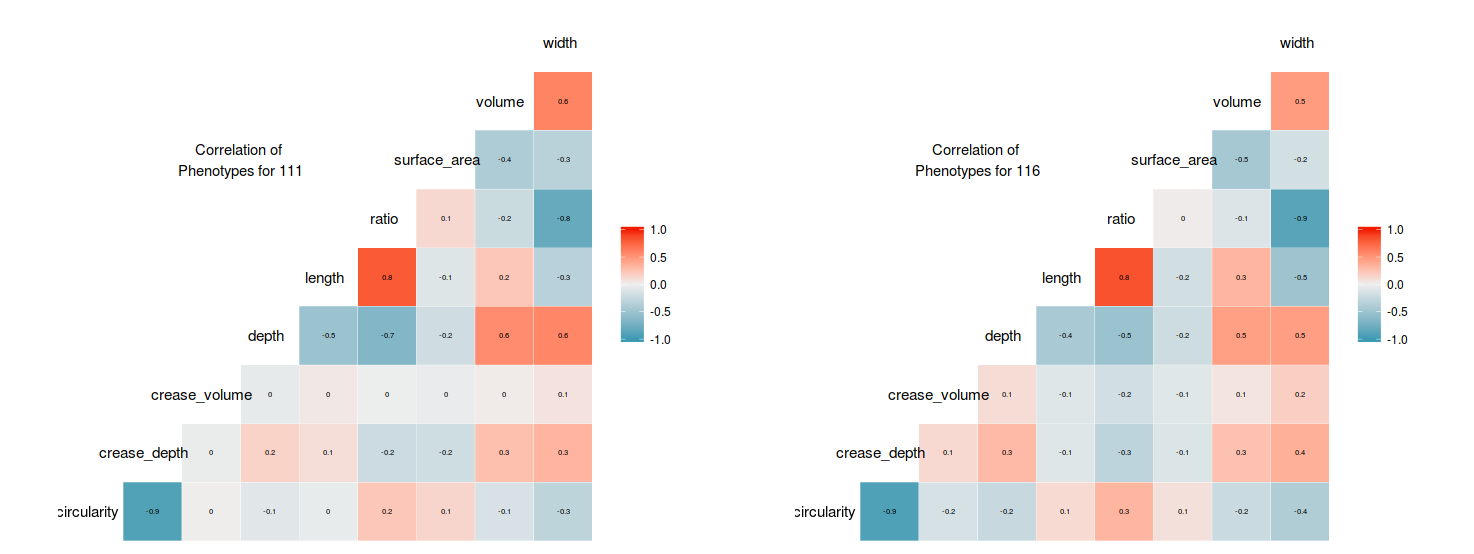
\includegraphics[width=14cm]{./corrmatrix.png}
\end{center}
\end{frame}

\section{Feedback from audience}
\label{sec:org8164a83}
\begin{frame}[label={sec:org9b78510}]{Feedback from audience}
\begin{block}{Suggested Models}
\begin{itemize}
\item Multiple Regressions
\item Simple linear models
\item More suggestions to use MANOVA
\end{itemize}
\end{block}
\begin{block}{Similar with the group's initial ideas}
\begin{itemize}
\item Which shows how different fields instinctively tackle/solve problems
\end{itemize}
\end{block}
\end{frame}


\section{Thanks}
\label{sec:org5336ef6}

\begin{frame}[label={sec:org9c92378}]{Thanks for listening!}
\begin{block}{Any Questions?}
\end{block}
\end{frame}
\end{document}
